\documentclass[11pt,a4paper]{article}
\usepackage[utf8]{inputenc}
\usepackage{amsmath, mathtools}
\usepackage{amsfonts, dsfont}
\usepackage{amssymb}
\usepackage{graphicx}
\usepackage{empheq}
\usepackage{bm}
\usepackage[round, sort]{natbib}
\usepackage{tikz}
\usepackage{mathtools}  
%\mathtoolsset{showonlyrefs}  
\usetikzlibrary{shapes,backgrounds,arrows,automata,snakes,shadows,positioning, mindmap}

%%%%% Commands
\newcommand{\argmin}{\arg\!\min}
\newcommand{\argmax}{\arg\!\max}
\newcommand*\widefbox[1]{\fbox{\hspace{3em}#1\hspace{3em}}}
\newcommand*\lesswidefbox[1]{\fbox{\hspace{2em}#1\hspace{2em}}}
\newcommand{\entr}{\mathcal{H}}
\newcommand{\betabf}{\boldsymbol{\beta}}
\newcommand{\thetabf}{\boldsymbol{\theta}}
\newcommand{\mubf}{\boldsymbol{\mu}}
\newcommand{\Omegabf}{\boldsymbol{\Omega}}
\newcommand{\Sigmabf}{\boldsymbol{\Sigma}}
\newcommand{\zerobf}{\boldsymbol{0}}
\newcommand{\Xbf}{\boldsymbol{X}}
\newcommand{\xbf}{\boldsymbol{x}}
\newcommand{\Ybf}{\boldsymbol{Y}}
\newcommand{\Zbf}{\boldsymbol{Z}}
\newcommand{\Sbf}{\boldsymbol{S}}
\newcommand{\mbf}{\boldsymbol{m}}
\newcommand\Ncal{\mathcal{N}}
\newcommand\Pcal{\mathcal{P}}
\newcommand\Tcal{\mathcal{T}} 
\newcommand{\Esp}{\mathds{E}}
\newcommand{\bound}{\mathcal{J}}
 
 %%%%%%% TIKZ
 \newcommand{\edgeunit}{1.5}
\providecommand\given{} % is redefined in \Set
\newcommand\SetSymbol[1][]{\nonscript\:#1\vert\nonscript\:}
%\usepackage[mathcal]{eucal}
\usepackage[left=2cm,right=2cm,top=2cm,bottom=2cm]{geometry}
\tikzset{%
    observed/.style={%
    scale=0.9,rectangle,draw=white,transform shape,fill=white,font=\Large}
}
\tikzset{%
    basic/.style={%
    scale=0.9,circle,draw=black,transform shape,fill=white,font=\small}
}


\setlength\parindent{0pt}
\author{Raphaelle Momal}
\title{PLN with missing actor}

 

\begin{document}

\maketitle
\vspace{3cm}
\tableofcontents
\newpage
Previously:
$$ p(\Ybf,\Zbf,T) = p(T)p(\Zbf|T)p(\Ybf|\Zbf)$$
$$ \Esp(\log p(\Ybf,\Zbf,T)|\Ybf) \approx \sum_{1 \leq j < k \leq p} P_{jk} \log\left(\beta_{jk} \hat{\psi}_{jk}\right) - \log B + cst$$

Now adding a hidden layer of unobserved data, indexed by H:

$$ p(\Ybf,\Zbf_O,\Zbf_H,T)$$
\section{PLNmissing peculiarities:}

\subsection{Model}

$$\left\{\begin{array}{rl}
T & \sim\prod_{jk \in T} \beta_{jk}/B \\\\
\Zbf|T& \sim\mathcal{N}(0,\Sigma_T)\\\\
\Ybf|\Zbf&\sim\mathcal{P}( \exp( \Xbf\theta^\intercal + \Zbf) )
\end{array} \right.$$

\paragraph{Dimensions:}
The model is build on matrices $\Ybf$ and $\Zbf$ with the following dimensions:\\
$\Ybf$: $n\times p$\\
$\Zbf_O$: $n\times p$\\
$\Zbf_H$: $n\times r$


\paragraph{Underlying dependencies:} This diagram is the graphical model behind the model, it describes the variables direct denpendencies and how data is simulated. Here, a tree $T$ is first drawn, which controls the dependency structure of parameters $\Zbf = (\Zbf_O,\Zbf_H)$. Count data $\Ybf$ is drawn from a distribution depending only on observed parameters $\Zbf_O$.
\begin{center}
	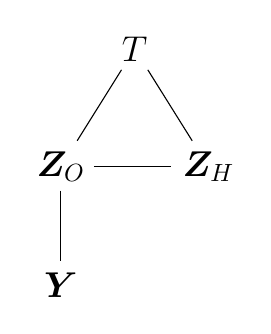
\begin{tikzpicture}	
      \tikzstyle{every edge}=[-,>=stealth',shorten >=1pt,auto,thin,draw]
		\node[observed] (A1) at (0.625*\edgeunit, 2*\edgeunit) {$T$};
		\node[observed] (A2) at (0*\edgeunit, 1*\edgeunit) {$\Zbf_O$};
		\node[observed] (A3) at (1.25*\edgeunit, 1*\edgeunit) {$\Zbf_H$};
		\node[observed] (A4) at (0*\edgeunit, 0*\edgeunit) {$\Ybf$};
		\path (A1) edge [] (A2)
        (A1) edge [] (A3)
        (A2) edge [] (A3)
        (A2) edge [] (A4);
	\end{tikzpicture}
\end{center}

\subsection{Distributions}
\label{distrib}
\paragraph{Marginals}
The complete vector of underlying parameters $Z$ follows a mixture of Gaussian laws on the space of all existing spanning trees.
\begin{align*}
(\Zbf_O,\Zbf_H) &\sim \sum_{T \in \mathcal{T}} p(T) \mathcal{N}(0,\Sigma_T) \\
\end{align*}

\paragraph{Conditional on T:}
Conditionally on the dependency structure $T$, $\Zbf$ is a centered Gaussian variable, with covariance matrix $\Sigma_T$ defined by block:
\[
 \Sigma=
  \left( {\begin{array}{cc}
  \Sigma_{TO} &  \Sigma_{TOH}\\\\
  \Sigma_{THO} & \Sigma_{TH}
  \end{array} } \right) =
   \left( {\begin{array}{cc}
  \Omega_{TO} &  \Omega_{TOH}\\\\
  \Omega_{THO} & \Omega_{TH}
  \end{array} } \right)^{-1}
  \]\\
This results in the following distributions:
\begin{align*}
(\Zbf_O,\Zbf_H)|T & \sim\mathcal{N}(0,\Sigma_T)\\
\Zbf_O|T & \sim\mathcal{N}(0,\Omega_{Tm}^{-1})\\
\end{align*}
With $ \Omega_{Tm} =\Sigma_{TO}^{-1} =  \Omega_{TO} - \Omega_{TOH}\Omega_{TH}^{-1}\Omega_{THO}$. This comes from the Schur's complement which is recalled in appendix.\\

A result from Lauritzen states that Gaussian precision matrices which are faithful to different trees will only differ in the position of their zero entries, meaning that any trees sharing  an edge will also share the same value in their precision matrix. Let's define $\Omega$ such as $$\forall T_a \in \{T \in\mathcal{T} / kl \in T \}, \Omega_{T_a}[k,l] =  \Omega [k,l].$$ Let's also define $I_T$ the binary matrix with diagonal one indicating the  edges presence in tree $T$ : $I_T=(\mathds{1}_{kl \in T} + \mathds{1}_{k=l})_{kl}$. Then we can write :
$$\forall T\in \mathcal{T}, \;\;\; \Omega_T = I_T \odot \Omega $$

For identifiability reasons, two hidden nodes cannot be linked with each. The $H$ bloc of $\Omega_T$ should thus be diagonal , and we get: 
\[
 \Omega_T=
  \left( {\begin{array}{cc}
 (I_T \odot \Omega)_O &  (I_T \odot \Omega)_{OH}\\\\
 (I_T \odot \Omega)_{HO} &   \Omega_H 
  \end{array} } \right) \]\\
  
  Note that the diagonal of $\Omega_T$ do not depend on $T$.
  
\paragraph{Conditional on observed data:\\}


As $\Zbf_O$ decouples $\Zbf_H$ and $\Ybf$, we will never need $\Zbf_H|\Ybf$:
$$ p(\Zbf|\Ybf) = p(\Zbf_O,\Zbf_H | \Ybf) = p(\Zbf_H|\Zbf_O) \: p(Z_O|\Ybf) $$




 In a precision matrix of a multivariate Gaussian, the conditional bloc is the marginal bloc:  $\Omega_{TH|O}^{-1} = \Sigma_{TH} -\Sigma_{THO}\Sigma_{TO}^{-1}\Sigma_{TOH} = \Omega_{TH}^{-1} =\Omega_{H}^{-1}$. Therefore the conditional distribution of the unobserved latent vectors given the latent observed ones is as follows: $$\Zbf_H|\Zbf_O,T \sim \mathcal{N}(\mu_{H|O,T}, \Omega_{H}^{-1})$$ 

  Let's $\Zbf_{Oi}$ denote a realization of $\mathcal{N}(0,\Sigma_{TO}) $. Then $\displaystyle  \mu_{H|Oi,T} = \Sigma_{THO}\Sigma_{TO}^{-1}(\Zbf_{Oi}-\underbrace{\mu_{\Zbf_Oi|T}}_{0}) 
 = -\Omega_{TH}^{-1}\Omega_{THO} \: \Zbf_{Oi}
$ 


\section{Variational EM inference}
\subsection{Approximation of the likelihood}
\paragraph{Joint likelihood:}
The graphical model gives the following writing of the joint likelihood:
\begin{align*}
p(\Ybf,Z,T)& = p(T) \: p(Z|T) \: p(\Ybf|Z) \\
&= p(T)\: p(Z_O,Z_H|T) \: p(\Ybf|Z_O,Z_H) \\
&= p(T) \: p(Z_O|T) \: p(Z_H | Z_O,T)  \: p(\Ybf|Z_O)
\end{align*} 


\paragraph{Variational approximation:}

Here $p(T,\Zbf \mid \Ybf)$ is untractable. We adopt a variational approximation aiming to maximise a lower bound of the log-likelihood of observed data $\log p(\Ybf)$, namely  
\begin{align*}
    \mathcal{J}(\Ybf; g,h)
    & = \log p(\Ybf) - KL\left[q(T,\Zbf) \middle\vert\middle\vert\ p(T,\Zbf \mid \Ybf)\right]
\end{align*}
Where KL is the Küllback-Leibler divergence. The approximation we adopt relies on factorizing $q$ in the product of two distributions $h$ and $g$ relating respectively to $\Zbf$  and $T$: 
$$p(T,Z | \Ybf) \approx  q(Z,T) = g(T)h(Z).$$

 A consequence of this hypothesis is the contributions of   $\Esp_h[\log p(\Zbf\mid T)]$ and $\log p(T)$ --~only terms involving $T$ in the lower bound~-- writing as sums on the edges. As distribution   $g$ minimizes the KL divergence, it has to factorizes on the edges as well and hence:
$ g(T) = \left(\prod_{kl} \widetilde{\beta}_{kl} \right) / \widetilde{B}$. \\
 
Moreover, it follows from the independence of the samples that $h$ is a product law: $ h(\Zbf) = \prod_i h_i(\Zbf_i)$.
Our variational approximation consists in assuming that each of its components is a multivariate Gaussian: $h(\Zbf_i) = \Ncal(\Zbf_i; \mbf_i, \Sbf_i)$, where $\Sbf_i$ is diagonal. More precisely:  $ h(Z_i) =  \mathcal{N}(m_i,S_i)$ , where $S_i$ is diagonal with diagonal $(s_{i1}^2, ... , s_{i(p+r)}^2)$, meaning that $\Zbf_H$ and $\Zbf_O$ are independent under distribution $h$. Marginals are written $h_O$  and  $h_H$. $S=\sum_i S_i$  and $ M =  [m_i]_{1 \leq i \leq (p+r)}$ (so $\Esp_h[Z_{\cdot k}^\intercal Z_{\cdot k}] = \sum_i s_{ik} + m_{\cdot k}^\intercal m_{\cdot k}$). $S$ is also diagonal and its H and O blocs are denoted $S_H$ and $S_O$. In the following, the $n\times p $ and $n\times r $ matrices $M_O$ and  $M_H$ compile all vectors of means $\mbf_i$ corresponding respectively to observed and hidden latent vectors ; $M_O$ and  $M_H$ are gathered in matrix $M= (M_O | M_H)$.

\textcolor{red}{SH is fixed}
%In the following we use the scalar product on the matrix space defined with the trace operator as: 
%$$  Tr(A^\intercal B) = <A,B> .$$
\paragraph{Lower bound:}
Starting with the two hidden layers of our model, the lower bound writes:
\begin{align*}
\mathcal{J}(\Ybf; g,h)&=\log p(\Ybf) - KL\left[g(T) h(\Zbf) \middle\vert\middle\vert\ p(T,\Zbf | \Ybf)\right]\\
&= \log p(\Ybf) - \Esp_{gh}[\log( g(T) h(\Zbf)) - \log p(\Zbf,T\mid \Ybf) ]\\
&= \log p(\Ybf) - \Esp_{gh}[\log g(T) + \log h(\Zbf) ] + \Esp_{gh}[\log p(\Ybf,\Zbf,T)] - \Esp_{gh}[\log p(\Ybf)]\\
&= \Esp_{gh} [\log p(\Ybf,\Zbf,T)] + \entr[g(T)] + \entr[h(\Zbf)]\\
&= \Esp_{gh} [\log (p_\beta(T)p_{\Omega}(\Zbf\mid T)p_\theta(\Ybf\mid \Zbf))] + \entr[g_{\widetilde{\beta}}(T)] + \entr[h_{M,S}(\Zbf)]
\end{align*}

Thus the model's parameters are $\Phi = (\beta, \Omega, \theta, \widetilde{\beta},M,S)$.
\subsection{Optimizing in $\theta$ and $h(\Zbf_O)$:}
\citet{CMR18} compute the lower bound of a VEM for the original PLN, which we write $\mathcal{J}_{PLN}$,  in the R package \textit{PLNmodels}. It is possible to use $\mathcal{J}_{PLN}$ in our computation as well, the following shows how.

Let's first separate observed and unobserved latent variables:
\begin{align*}
\mathcal{J}(\Ybf; g,h)&= \Esp_{gh}[\log p(T)  p(\Zbf_H| \Zbf_O,T) p(\Zbf_O|T)p(\Ybf|\Zbf_O)] + \entr[g(T)] +\entr[h(\Zbf_H,\Zbf_O)]
\end{align*}

 We develop the entropy of the complete $\Zbf$ vector, to make the entropy of $\Zbf_O$ appear. $\Zbf_O$ and $\Zbf_H$ being independant under the $h$ distribution, we have:
\begin{align*}
\entr[h(\Zbf_H,\Zbf_O)] &= -\Esp_h[\log h(\Zbf_H,\Zbf_O)] =-\Esp_h[\log h(\Zbf_H)] - \Esp_h[\log \Zbf_O)]\\
&=\entr[h(\Zbf_O)] +\entr[h(\Zbf_H)]
\end{align*}

Now using the hypothesis of independence of $g$ and $h$, we can obtain quantities with separate dependencies:
\begin{align}
\mathcal{J}(\Ybf; g,h)&=  \Esp_{gh}[\log p(\Zbf_O | T)] +\Esp_h[\log p(\Ybf|\Zbf_O)]+\entr[h(\Zbf_O)]  \label{PLNlike}\\
& \;\; + \Esp_{gh}[\log p(\Zbf_H | \Zbf_O,T) ]+\Esp_g[\log p(T)] +\entr[g(T)]+\entr[h(\Zbf_H)] \label{new}
\end{align}

Let's then detail the first term of the lower bound:
\begin{align*}
\Esp_{gh}[\log p(\Zbf_O|T)] &=  \Esp_{gh} \left[\frac{n}{2} \log |\Omega_{Tm}| - \frac{1}{2} \sum_i \Zbf_{Oi}\Omega_{Tm} \Zbf_{Oi}^\intercal  \right]\\
&= \frac{n}{2} \Esp_g [\log |\Omega_{Tm}|] - \frac{1}{2} \Esp_{gh}\left[Tr\left( \Zbf_O^\intercal \Zbf_O \Omega_{Tm}\right)\right].
\end{align*}

The expectation in $gh$ is again separable thanks to the independence hypothesis. As the trace is a linear operation we obtain:
\begin{align*}
\Esp_{gh}[\log p(\Zbf_O|T)] &=\frac{n}{2} \Esp_g [\log |\Omega_{Tm}|] - \frac{1}{2}  Tr\left(\Esp_h [\Zbf_O^\intercal \Zbf_O ]\; \Esp_g[\Omega_{Tm}]\right) 
\end{align*}
$\Esp_g [\Omega_{Tm}]$ is a $p\times p$ matrix of expected inverse covariance over the whole spanning-tree space. Introducing the quantity  $\log |\Esp_g [\Omega_{Tm}]| $ in part (\ref{PLNlike}) of $\mathcal{J}(\Ybf; g,h)$:
\begin{align*}
&\Esp_{gh}[\log p(\Zbf_O | T)] +\Esp_h[\log p(\Ybf|\Zbf_O)]+ \entr[h(\Zbf_O)]\\
& =\ \frac{n}{2} \log |\Esp_g [\Omega_{Tm}]| - \frac{1}{2}Tr\left(\Esp_h [\Zbf_O^\intercal \Zbf_O ]\; \Esp_g[\Omega_{Tm}]\right)+ \Esp_{h}[\log p(\Ybf|\Zbf_O)] + \entr[h(\Zbf_O)]\\
& \;\;\;+  \frac{n}{2}\left( \Esp_g[\log|\Omega_{Tm}|] - \log|\Esp_g [\Omega_{Tm}]|\right)
\end{align*}
%The second line is a negative quantity, because the log determinent is a concave function. Jensen's inequality gives:
%$$\log |\Esp_g[\Omega_{Tm}]| \geq \Esp_g [\log |\Omega_{Tm}|]$$
%$$ \Esp[Z_jZ_k] = -\partial_{\omega_{jk}}( \log |\Omega_{TO}| )$$
%Therefore,
Assuming $\Esp_g [\Omega_{Tm}]$ is an inverse variance covariance matrix for $\Zbf_O$, the lower bound $\mathcal{J}_{PLN}$ appears:
 $$\Esp_{gh}[\log p(\Zbf_O | T)] +\Esp_h[\log p(\Ybf|\Zbf_O)]+ \entr[h(\Zbf_O)] = \mathcal{J}_{PLN} - \frac{n}{2}\left( \Esp_g[\log|\Omega_{Tm}|] - \log|\Esp_g [\Omega_{Tm}]|\right)$$
 
As the last term do not depend either on $\theta$ or $h(\Zbf_O)$, we finally obtain that
 $$ \argmax_{\theta, h(\Zbf_O)} \big\{\Esp_{gh}[\log p(\Zbf_O | T)] +\Esp_h[\log p(\Ybf|\Zbf_O)]+ \entr[h(\Zbf_O)]\big\} = \argmax_{\theta, h(\Zbf_O)} \big\{ \mathcal{J}_{PLN} \big\}.$$

The VE step of PLNmodels VEM algorithm maximizes $\mathcal{J}_{PLN}$ and gives estimates of $\Zbf_O$ moments of order 1 and 2, so we have easy access to estimates $\widetilde{M}_O$ and $\widetilde{S}_O$. As there are still some dependence in $h(\Zbf_O)$ in part (\ref{new}) of $\mathcal{J}(\Ybf; g,h)$, using $\argmax_{\theta, h(\Zbf_O)} \big\{ \mathcal{J}_{PLN} \big\}$ maximizes  $\mathcal{J}(\Ybf;g,h)$ in $\theta$, and only partly in $h(\Zbf_O)$. Therefore   the proposed solution is sub-optimal. \\

After maximizing part (\ref{PLNlike}) of $\mathcal{J}(\Ybf; g,h)$ in $h_O$, this density is considered constant and written $h_O^*$.  We can then write the partly optimized  lower bound as follows:
\begin{align*}
\mathcal{J}_{h_O^*}(\Ybf; g,h)&= \Esp_{h_O^*}[\log p(\Ybf \mid \Zbf_O)] - \Esp_{h_O^*}[\log h(\Zbf)] + \Esp_{gh}[\log p(\Zbf \mid T)] + \Esp_g \big[\log p(T) - \log g(T) \big]
\end{align*}

 Note that $\Esp_{h_O^*}[\log h(\Zbf)]$ is now completely optimized in $h$, as it is a Gaussian entropy therefore only depending on its variance, and that $S_H$ is considered constant for identifiability reasons.

\paragraph{About $\Esp_g [\Omega_{Tm}]$:}
Here it shows that assuming a tree structure for the latent layer of parameters $\Zbf$ reveals an average precision matrix over all the precision matrices of possible trees.  Recalling the writing of $\Omega_T$ of sub-section \ref{distrib}, we have that
 \begin{align*}
 \Esp_g [\Omega_{T}] & = \Esp_g [I_T \odot \Omega ] = \Esp_g [I_T] \odot \Omega \\
 &= P_g\odot \Omega
 \end{align*}

Where $P_g$ is the matrix of edge probabilities under the $g$ distribution. For a specific edge $kl$, we indeed have that $\Esp_g [I_T[k,l]] = \Esp_g [\mathds{1}_{kl \in T}] =  \sum_{\substack{T\in \mathcal{T}\\ kl \in T } }g(T) = P_g[k,l]$.

The lower bound of \cite{CMR18} normally involves $\Sigma_O^{-1}$. Thus using it in our context yields the following approximation:
$$\Sigma_O^{-1} \approx \Esp_g[\Omega_{Tm}] = (P_g \odot \Omega_m)[O,O] $$

\textcolor{red}{Study $\Delta =\Sigma_O^{-1} -   (P_g \odot \Omega_m)[O,O]$ }
\subsection{VE step: optimizing in $g$ and $h(\Zbf_H)$}
The VE step minimizes the Küllback-Leibler divergence between the approximated and the aimed distributions :

$$  \argmin_{g,h(\Zbf_H)} KL\left(g(T)h(\Zbf) \mid\mid p(\Zbf,T|\Ybf)\right)$$


\begin{align*}
KL\left(g(T)h(\Zbf) \mid\mid  p(\Zbf,T|\Ybf)\right) &= \Esp_{gh}\left[\log g(T)h(\Zbf) - \log p(\Zbf,T\mid \Ybf) \right]\\
&= \Esp_{gh}\left[\log g(T)h(\Zbf) - \log p(\Ybf,\Zbf,T) + \log p(\Ybf)  \right]\\
&= \Esp_{gh}\left[\log g(T)+ \log h(\Zbf) - \log (p(T)p(\Zbf\mid T) p(\Ybf\mid \Zbf_O)) + \log p(\Ybf)  \right]\\
&= -\Esp_{gh}[\log p(\Zbf \mid T) ] - \Esp_g[\log p(T) - \log g(T)] - \entr[h(\Zbf)]\\
& \;\;\;\; -\Esp_h[\log p(\Ybf \mid \Zbf_O)] +\log p(\Ybf) 
\end{align*}
Distributions $p(\Ybf)$ and $p(\Ybf\mid \Zbf_O)$  do not depend on distributions $g$ and $h(\Zbf_H)$. Moreover, $\entr[h(\Zbf)]$ does not need to be optimized in $h(\Zbf_H)$ as $S_H$ stays constant. We obtain:
 
\begin{empheq}[box=\widefbox]{align*}
\argmin_{g,h(\Zbf_H)} KL  &=\argmin_{g,h(\Zbf_H)} \Big\{ -\Esp_{gh}[\log p(\Zbf \mid T) ] - \Esp_g[\log p(T) - \log g(T)]\Big\}
\end{empheq}
 
 During the minimization, we will use the optimized distribution $h(\Zbf_O^*) = \prod_i^n \mathcal{N}(\widetilde{\mbf}_{Oi}, \widetilde{S}_{Oi})$, its parameters being gathered in $n\times p$ matrices $\widetilde{M}_O$ and $\widetilde{S}_O$.
 
\subsubsection{Details of  $\Esp_{gh}[\log p(\Zbf \mid T) ]$} 
 $$\log p(\Zbf \mid T) = \frac{n}{2} \log |\Omega_T| - \frac{1}{2} Tr(\Omega_T \times \Zbf^\intercal \Zbf) $$
 Taking the expectation, and by independence of $g$ and $h$:
 $$\Esp_{gh} [\log(\Zbf \mid T)] = \frac{n}{2} \Esp_{gh} [\log | \Omega_T|] - \frac{1}{2} Tr(\Esp_g[\Omega_T] \Esp_h[\Zbf^\intercal \Zbf])$$
 
\paragraph{Determinant of $\Omega_T$\\}
Because $\Omega_{T}$ is tree-structured, its determinant factorizes on the edges of $T$. More precisely as in \citet{robin2019}:
\begin{align*}
|\Omega_{T}| &= \prod_{k=1}^{(p+r) }\omega_{kk} \prod_{kl \in T} \frac{\omega_{kk}\omega_{ll}-\omega_{kl}^2}{\omega_{kk}\omega_{ll}}\\
\log |\Omega_{T}|&= \sum_{k} \log \omega_{kk} + \sum _{k<l} \mathds{1}\{kl \in T\} \left[\log\frac{\omega_{kk}\omega_{ll}-\omega_{kl}^2}{\omega_{kk}\omega_{ll}}\right]
\end{align*}
Each edge is only counted once in the sum on edges above. Defining $\varphi_{kl} = 1- \frac{\omega_{kl}^2}{\omega_{kk}\omega_{ll}}$ and $P_{kl} = \mathds{P}_g\{kl \in T \}$, we obtain:

$$\Esp_g[\log |\Omega_{T}|]= \frac{1}{2}\sum _{kl} P_{kl} \log (\varphi_{kl}) + \sum_{k} \log \omega_{kk} $$ 

\paragraph{Expectation of $\Zbf^\intercal \Zbf$\\}
The definition of variance gives:
\begin{align*}
\Esp_h[\Zbf^\intercal \Zbf] &= \Esp_h[\Zbf]^\intercal \Esp_h[\Zbf] + \mathds{V}_h(\Zbf)\\
& = M^\intercal M + S\\
&= n \times \widetilde{\Sigma}
\end{align*}
So we have 
\begin{align*}
Tr(\Esp_g[\Omega_T] \Esp_h[\Zbf^\intercal \Zbf]) &= n \times Tr( (P\odot \Omega)\widetilde{\Sigma})
\end{align*}

Finally:

\begin{empheq}[box=\widefbox]{align*}
\Esp_{gh} [\log(\Zbf \mid T)] = \frac{n}{2} \Big( \sum_{k} \log \omega_{kk}+\frac{1}{2}\sum _{kl} P_{kl} \log (\varphi_{kl}) - \sum_{kl} P_{kl} \omega_{kl} \widetilde{\sigma}_{kl} - \sum_{h \in H} \omega_{hh} \widetilde{\sigma}_{hh}\Big)
 \end{empheq}

\subsubsection{Details of $\Esp_g[\log g(T) - \log p(T)]$}
\begin{align*}
\log g(T) - \log p(T) &= \left(  \sum_{jk} \mathds{1}\{jk \in T\} \log \widetilde{\beta}_{jk} - \log \widetilde{B}\right) - \left(  \sum_{jk} \mathds{1}\{jk \in T\} \log {\beta}_{jk} - \log {B}\right)\\
&=\sum_{jk} \mathds{1}\{jk \in T\} \log \frac{\widetilde{\beta}_{jk}}{{\beta}_{jk}} - \log \frac{\widetilde{B}}{B}
\end{align*}
$$\boxed{
\Esp_g[\log g(T) - \log p(T)] = \sum_{jk}P_{gjk} \left(\log \frac{\widetilde{\beta}_{jk}}{{\beta}_{jk}}\right) - \log \frac{\widetilde{B}}{B} }$$

 
This is also the (opposite of the) Kullback–Leibler divergence of a tree drawn under $p$ from a tree draw under $g$. This can be used in network comparison.


\subsubsection{Details of $\Esp_h[\log h(\Zbf_H\mid \Zbf_O)]$}
Under $h$, $\Zbf_H$ and $\Zbf_O$ are independent according to our variational approximation. Therefore, $h(\Zbf_H\mid \Zbf_O) = h(\Zbf_H)$ and this terms boils down to the entropy of $h(\Zbf_H)$. More precisely:

\begin{align*}
\Esp_h[\log h(\Zbf_H\mid \Zbf_O)] &= \Esp_{h(\Zbf_O)}\left[\Esp_{h(\Zbf_H\mid \Zbf_O)}[\log h(\Zbf_H\mid \Zbf_O)]\right]\\
&=\Esp_{h(\Zbf_O)}\left[\Esp_{h(\Zbf_H)}[\log h(\Zbf_H)]\right]\\
&=\Esp_{h(\Zbf_H)}[\log h(\Zbf_H)]  
\end{align*}


Now $\Zbf_{Hi} \sim \mathcal{N}(m_{Hi},S_{ih})$ and $h$ is a product law on all $\Zbf_{Hi}$. Therefore, recalling the entropy of a multivariate Gaussian:
\begin{align*}
\Esp_h[\log h(\Zbf_H\mid \Zbf_O)]  &= - \entr[h(\Zbf_H)] \\
&= -\sum_i \entr[h(\Zbf_{Hi})] \\
&=-\frac{1}{2} \sum_i\log |S_{Hi}| -\underbrace{n\times  \frac{r}{2}(1+\log(2\pi))}_{cst}\\
&= -\frac{1}{2} \sum_i \log \left(\prod_{h=1}^r S_{Hi}[h,h] \right)-cst\\
&= -\frac{1}{2}\sum_{i=1}^n \sum_{h=1}^r \log(s_{hi}^2)-cst
\end{align*}
Finally $$\boxed{ \Esp_h[\log h(\Zbf_H\mid \Zbf_O)] = -\frac{1}{2}\sum_{i=1}^n \sum_{h=1}^r \log(s_{hi}^2) -cst}.$$

\subsubsection{Final quantity to optimize:}
\begin{align*}
\argmin_{g,h(\Zbf_H)} KL  &=\argmin_{g,h(\Zbf_H)}  \Big\{- \Esp_{gh}[ p(\Zbf_H|\Zbf_O,T)] - \Esp_{gh_O^*}[\log p(\Zbf_O|T)] + \Esp_g\big[\log g(T)-\log p(T)\big]\\
& \hspace{2.5cm} + \Esp_h[\log h(\Zbf_H)]  \Big\}\\
&= \argmin_{g,h(\Zbf_H)}  \bigg\{ -\frac{n}{2} \log |\Omega_H| + \frac{1}{2}<\Omega_H, M_H^\intercal M_H + S_H> + <\Esp_g[\Omega_{TOH}],M_H^\intercal \widetilde{M}_O> \\
& \;\;\;+ \frac{1}{2}<\Esp_g\big[\Omega_{TOH}\Omega_H^{-1}\Omega_{THO}\big],\widetilde{M}_O^\intercal \widetilde{M}_ O + \widetilde{S}_ O> -\frac{n}{2}\sum_{k\in O} \log \omega_{kk}+\sum _{kl} P_{gkl}  \log\left(1- \frac{ \omega_{kl}^2}{\omega_{kk}\omega_{ll}}\right)^{-\frac{n}{2}} \\
&  \;\;\;+ \frac{1}{2}<\Esp_g[\Omega_{TO}],\widetilde{M}_O^\intercal \widetilde{M}_O + \widetilde{S}_O> - \frac{1}{2}<\Esp_g\big[\Omega_{TOH}\Omega_H^{-1}\Omega_{THO}\big],\widetilde{M}_O^\intercal \widetilde{M}_O + \widetilde{S}_O> \\
& \;\;\; + \sum_{jk}P_{gjk} \left(\log \frac{\widetilde{\beta}_{jk}}{{\beta}_{jk}}\right) - \log \frac{\widetilde{B}}{B} -\frac{1}{2}\sum_{i=1}^n \sum_{h=1}^r \log(s_{hi}^2)\bigg\}
\end{align*}

Above, the two terms involving $\Esp_g\big[\Omega_{TOH}\Omega_H^{-1}\Omega_{THO}\big]$ simplify, and the $\log |\Omega_H|$ get into the sum of diagonal terms, as $\Omega_H$ is diagonal by hypothesis. Finally, the optimization task is:
\begin{empheq}[box=\widefbox]{align*}
&\argmin_{g,h(\Zbf_H)}  \bigg\{\frac{1}{2}<\Omega_H, M_H^\intercal M_H + S_H> + <\Esp_g[\Omega_{TOH}],M_H^\intercal \widetilde{M}_O> + \frac{1}{2}<\Esp_g[\Omega_{TO}],\widetilde{M}_O^\intercal \widetilde{M}_O + \widetilde{S}_O>\\
& \;\;\; -\frac{n}{2}\sum_{k} \log \omega_{kk}+\sum _{kl} P_{gkl}  \log\left(1- \frac{ \omega_{kl}^2}{\omega_{kk}\omega_{ll}}\right)^{-\frac{n}{2}}   + \sum_{jk}P_{gjk} \left(\log \frac{\widetilde{\beta}_{jk}}{{\beta}_{jk}}\right) - \log \frac{\widetilde{B}}{B} -\frac{1}{2}\sum_{i=1}^n \sum_{h=1}^r \log(s_{hi}^2)\bigg\}\\
\end{empheq}

\subsubsection{Update formula for $\widetilde{\beta}$ }
In the following we denote  $\varphi = \left( 1-\frac{\omega_{kl}^2}{\omega_{kk}\omega_{ll}} \right)^{-\frac{n}{2}}$. From the quantity to be minimized, we need terms depending on the edges, as $\widetilde{\beta}$ are defined up to an additive constant. These terms are those  which involve edges probabilities:
\begin{align*}
& <\Esp_g[\Omega_{TOH}],M_H^\intercal \widetilde{M}_O> + \frac{1}{2}<\Esp_g[\Omega_{TO}],\widetilde{M}_O^\intercal \widetilde{M}_O + \widetilde{S}_O>+\sum _{kl} P_{gkl}  \log\left(1- \frac{ \omega_{kl}^2}{\omega_{kk}\omega_{ll}}\right)^{-\frac{n}{2}}   + \sum_{jk}P_{gjk} \left(\log \frac{\widetilde{\beta}_{jk}}{{\beta}_{jk}}\right)\\
&=Tr(P_g\odot\Omega_{OH}M_H^\intercal \widetilde{M}_O) + \frac{1}{2} Tr(Pg\odot \Omega_O (\widetilde{M}_O^\intercal \widetilde{M}_O + \widetilde{S}_O) ) + \sum_{kl} P_{gkl} \log \left( \varphi_{kl} \widetilde{\beta}_{kl}/\beta_{kl} \right)\\
&= \sum_{kh \in O\times H} P_{gkh} \times \omega_{kh} [M_H^\intercal \widetilde{M}_O]_{hk} + \frac{1}{2} \sum_{kl \in O^2} P_{gkl} \times \omega_{kl} [\widetilde{M}_O^\intercal \widetilde{M}_O + \widetilde{S}_O]_{kl}]+ \sum_{kl \in (O+H)^2} P_{gkl} \log \left( \varphi_{kl} \widetilde{\beta}_{kl}/\beta_{kl} \right) \\
\end{align*}
 
Setting the above quantity to zero to get an expresison for $\widetilde{\beta}$, we obtain:
 
\[\left\{\begin{array}{ll r}
\widetilde{\beta}_{jk} &= \frac{\beta_{jk}}{\varphi_{jk}}\exp\Big(-\frac{1}{2} \omega_{jk}[\widetilde{M}_O^T \widetilde{M}_O]\Big) & ,jk \in O\times O\\
\widetilde{\beta}_{kh} &=\frac{\beta_{kh}}{\varphi_{kh}}\exp\Big(-\frac{1}{2} \omega_{kh}[\widetilde{M}_H^T \widetilde{M}_O]\Big) & ,kh \in O\times H
\end{array}\right.\]
 

The matrix $\widetilde{\betabf}$ allows us to build an approximate of the distribution of a tree $T$ conditional to  data $\Ybf$:
$$\tilde{p}(T|\Ybf) = \prod_{kl} \widetilde{\beta}_{kl} \big/ D $$
where $D = \sum_{T\in \mathcal{T}}\prod_{kl} \widetilde{\beta}_{kl}$ is the normalisation constant. As distribution $g$ aim is to approach the condiitonal distribution of $T$, we can write:
\begin{align*}
\mathds{P}_g(kl \in T) &\simeq 1 - \sum_{T : kl \notin T}  \tilde{p}(T|\Ybf)\\
&= 1 - \frac{1}{D} \sum_{T : kl \notin T}\prod_{kl} \widetilde{\beta}_{kl}
\end{align*}

This sum-product quantity is computationaly available thanks to the Matrix Tree theorem. We therefore compute:
$$\boxed{P_{gkl}^{h+1} = 1 - \dfrac{|Q_{uv}^*(\widetilde{\betabf}_{\setminus kl}^h)|}{|Q_{uv}^*(\widetilde{\betabf}^h)|} \simeq\mathds{P}_g(kl \in T)}$$

\subsubsection{Final derivatives and optimal estimators}

At step $(t+1)$ of the VE part of the algorithm, the following updates occur:
\paragraph{$M_H$:}
\begin{align*}
\partial_{M_H} KL &= M_H\Omega_H  + \widetilde{M}_O(P_{gOH}\odot\Omega_{OH}) =0\\
\iff& \boxed{M_H^{t+1} =- \widetilde{M}_O(P_{gOH}^t\odot\Omega_{OH})\Omega_H^{-1}}
\end{align*}


\paragraph{$S_H$:}
\begin{align*}
\frac{1}{2}<\Omega_H, S_H> &= \frac{1}{2} \sum_h \omega_{hh}\sum_i s_{ih}^2\\
\end{align*}
\begin{align*}
\partial_{s_{ih}^2} KL &=  \frac{\omega_{hh}}{2}- \frac{1}{2s_{ih}^2} = 0\\
\iff & \boxed{s_{ih}^2 = \frac{1}{\omega_{hh}}}
\end{align*}


\paragraph{$\widetilde{\beta}$:}

\[\left\{\begin{array}{ll r}
&\boxed{\widetilde{\beta}_{jk} =\frac{\beta_{jk}}{\varphi_{jk}}\exp\Big(-\frac{1}{2} \omega_{jk}[\widetilde{M}_O^T \widetilde{M}_O]\Big) }& ,jk \in O\times O\\
&\boxed{\widetilde{\beta}_{kh} =\frac{\beta_{kh}}{\varphi_{kh}}\exp\Big(-\frac{1}{2} \omega_{kh}[\widetilde{M}_H^T \widetilde{M}_O]\Big) }& ,kh \in O\times H
\end{array}\right.\]

\subsection{M step: optimizing in $(\beta, \Omega)$}
 
$$ \argmax_{\beta, \Omega} \mathcal{J}(\Ybf ; g,h) =\argmax_{\beta, \Omega} \left\{ \Esp_{gh} [\log (p_\beta(T)p_{\Omega_T}(\Zbf\mid T) ]\right\} $$

\subsubsection{General expression}
\begin{align*}
\log (p_\beta(T)p_{\Omega_T}(\Zbf\mid T))  &= \sum_{kl} \mathds{1}\{kl \in T\} \log \beta_{kl} - \log B + \frac{n}{2}\log |\Omega_T| - \frac{1}{2}<\Omega_T,\Zbf^\intercal \Zbf>\\
\Esp_{gh} [\log (p_\beta(T)p_{\Omega_T}(\Zbf\mid T) ] &= \sum_{kl} P_{gkl} \log\beta_{kl} +\frac{n}{2} \Esp_g[\log |\Omega_T|] -\frac{1}{2} <\Esp_g [\Omega_T], \Esp_h[\Zbf^\intercal \Zbf]>- \log B
\end{align*}

$\Omega_T$ is tree-strucutred, so its determinent is decomposable on the edges:
$$|\Omega_{T}| = \prod_{k} \omega_{kk} \prod_{kl \in T} \frac{\omega_{kk}\omega_{ll}-\omega_{kl}^2}{\omega_{kk}\omega_{ll}}$$

And we get

$$\Esp_g[\log |\Omega_{T}|]= \sum _{kl} P_{gkl} \left[ \log\left(\frac{\omega_{kk}\omega_{ll}-\omega_{kl}^2}{\omega_{kk}\omega_{ll}}\right)\right] + \sum_k \log \omega_{kk}$$

Finally, denoting $\psi_{kl} = \left(\frac{\omega_{kk}\omega_{ll}-\omega_{kl}^2}{\omega_{kk}\omega_{ll}}\right)^{n/2}$ we obtain:
\begin{align*}
\Esp_{gh} [\log (p_\beta(T)p_{\Omega_T}(\Zbf\mid T) ] &=\sum_{kl} P_{gkl} \left(\log  \beta_{kl}\psi_{kl}\right) + \frac{n}{2}\sum_k \log \omega_{kk} - \frac{1}{2}<P_g \odot \Omega, \widetilde{M}^\intercal \widetilde{M} + \widetilde{S}>- \log B
\end{align*}
 
\subsubsection{Update formulas}
\paragraph{Update of $\beta$:}
\begin{align*}
\partial_{\beta_{jk}} \Esp_{gh} [\log (p_\beta(T)p_{\Omega_T}(\Zbf\mid T) ] &= \frac{P_{gjk}}{\beta_{jk}} - \frac{\partial_{\beta_{jk}} B }{B} \\
&=\frac{P_{gjk}}{\beta_{jk}}  - [M(W)]_{jk} \\
=0 \iff & \boxed{\widehat{\beta}_{jk} = P_{gjk} / ([M(W)]_{jk})}
\end{align*}\\


\paragraph{Update of $\Omega$:}

\[
 \partial_{\omega_{kl}}\left(\sum_{kl} P_{gkl} \left(\log  \beta_{kl}\psi_{kl}\right) +\frac{n}{2} \sum_k \log \omega_{kk}\right) =\begin{cases}
               -n \frac{P_{gkl} }{\omega_{kk}\omega_{ll}-\omega_{kl}^2}\times \omega_{kl} \text{\hspace{1cm}if $k\neq l$}\\\\
              \frac{n}{2} \times\frac{1}{\omega_{kk}} \left(\sum_l P_{gkl} \frac{\omega_{kl}^2}{(\omega_{kk}\omega_{ll}-\omega_{kl}^2)} + 1\right)\text{\hspace{0.5cm}if $k = l$}
            \end{cases}
\]
And
\begin{align*}
- \frac{1}{2} <P_g \odot \Omega, \underbrace{\widetilde{M}^\intercal \widetilde{M} + \widetilde{S}}_{n\widetilde{\Sigma}}> &=- \frac{n}{2}\times 2 \times \sum_{j<k}P_{gjk} \omega_{jk} \widetilde{\sigma}_{jk}- \frac{n}{2}\sum_{ k} \omega_{kk} \widetilde{\sigma}_{kk}
\end{align*}
The "$\times 2$" above comes from differenciating $j$ from $k$.
\begin{itemize}

\item The complete derivative for off-diagonal terms of $\Omega$ is :
\begin{align*}
 \partial_{\omega_{kl}}\Esp_{gh} [\log (p_\beta(T)p_{\Omega_T}(\Zbf\mid T) ] &=-n \frac{P_{gkl} }{\omega_{kk}\omega_{ll}-\omega_{kl}^2}\times \omega_{kl} - n P_{gjk}  \widetilde{\sigma}_{jk} =0\\
 \iff & \widetilde{\sigma}_{jk} \omega_{kl}^2 - \omega_{kl} - \widetilde{\sigma}_{jk} \omega_{kk}\omega_{ll} = 0 \\
 \iff & \widehat{\omega}_{kl} = (1 \pm \sqrt{1+4\widetilde{\sigma}_{jk}^2 \omega_{kk}\omega_{ll}}) / 2\widetilde{\sigma}_{jk}
\end{align*}

To choose between roots, we use the constraint $\dfrac{\omega_{kl}^2}{\omega_{kk}\omega_{ll}} < 1$ which is equivalent to 
$$ (1 \pm \sqrt{1+4\widetilde{\sigma}_{jk}^2 \omega_{kk}\omega_{ll}}) < 4\widetilde{\sigma}_{jk}^2 \omega_{kk}\omega_{ll}.$$
As $\widetilde{\sigma}_{jk}^2 \omega_{kk}\omega_{ll} > 0$ by positive-definitiveness of $\Omega$, we have:
\begin{align*}
&1 - \sqrt{1+4\widetilde{\sigma}_{jk}^2 \omega_{kk}\omega_{ll}} < 1- \sqrt{4\widetilde{\sigma}_{jk}^2 \omega_{kk}\omega_{ll}}\\
\iff &(1 - \sqrt{1+4\widetilde{\sigma}_{jk}^2 \omega_{kk}\omega_{ll}})^2 < ( \sqrt{4\widetilde{\sigma}_{jk}^2 \omega_{kk}\omega_{ll}}-1)^2 < 4\widetilde{\sigma}_{jk}^2 \omega_{kk}\omega_{ll}
\end{align*}

On the other hand, we also have:
\begin{align*}
&(1 + \sqrt{1+4\widetilde{\sigma}_{jk}^2 \omega_{kk}\omega_{ll}})^2 >4\widetilde{\sigma}_{jk}^2 \omega_{kk}\omega_{ll}.
\end{align*}

Therefore: $$\boxed{ \widehat{\omega}_{kl} = (1 - \sqrt{1+4\widetilde{\sigma}_{jk}^2 \omega_{kk}\omega_{ll}}) / 2\widetilde{\sigma}_{jk}}$$


\item We get the complete derivative for diagonal terms of $\Omega$:
\begin{align*}
 \partial_{\omega_{kk}}\Esp_{gh} [\log (p_\beta(T)p_{\Omega_T}(\Zbf\mid T) ] &=\frac{n}{2} \times\frac{1}{\omega_{kk}} \left(\sum_l P_{gkl} \frac{\omega_{kl}^2}{(\omega_{kk}\omega_{ll}-\omega_{kl}^2)} + 1\right) -\frac{n}{2}\widetilde{\sigma}_{kk} =0\\
 \iff &  \frac{1}{\omega_{kk}} \left(\sum_l P_{gkl} \frac{\omega_{kl}^2}{(\omega_{kk}\omega_{ll}-\omega_{kl}^2)} + 1\right) =\widetilde{\sigma}_{kk}
\end{align*}
Then from the optimization of the off-diagonal terms, we have that $$\frac{\omega_{kl}}{(\omega_{kk}\omega_{ll}-\omega_{kl}^2)}  = - \widetilde{\sigma}_{kl}  $$

which leads to 
$$\boxed{ \hat{\omega}_{kk} = \frac{1}{\widetilde{\sigma}_{kk}} \left( 1- \sum_l  P_{gkl} \;\omega_{kl} \;\widetilde{\sigma}_{kl}\right)}$$
\end{itemize}

\section{Model selection criteria}

A variational lower bound of the BIC criteria is available. The true BIC is defined as:
$$ BIC = \log p(\Ybf) - \frac{D}{2} \log(n) $$
where D is the number of parameters to estimate. A variational version of this is 
$$vBIC = \bound(\Ybf; g,h) - \frac{D}{2} \log(n)  $$

Our model estimates regression parameters, weights $\beta$ and the $\Omega$ matrix, which yields
$$D = p(d+1) + p(p-1)/2 + p(p+1)/2 $$
if we estimate the diagonal of $\Omega$ as well.
Now suppose we assume $r$ missing actors. The terms of the diagonals of matrices $\beta$ and $\Omega$ corresponding to missing actors are fixed. As these matrices are symmetrical,  there are $pr$ more parameters to estimate in both of them. Therefore the BIC variational lower bound for $r$ missing actors is
$$ vBIC_r=\bound_r(\Ybf; g,h) - \frac{D+2pr}{2} \log(n)  $$
 
%%%%%%%%%%%%%%%%%%%%%%%%%%%%%%%%%%%%%%%%%%%%% 
\newpage
\bibliographystyle{apsrev} %tested plainnat
\bibliography{bibi}

\appendix
\section{Technical material}
\subsection{Schur's complement}
\begin{align*}
 \Sigma_T=
  \left( {\begin{array}{cc}
  \Omega_{TO} &  \Omega_{TOH}\\\\
  \Omega_{THO} & \Omega_{TH}
  \end{array} } \right)^{-1} &=
  \left( {\begin{array}{cc}
  \Sigma_{TO} =( \Omega_{TO} - \Omega_{THO}\Omega_{TH}^{-1}\Omega_{TOH})^{-1} &  - \Sigma_{TO} \Omega_{TOH}\Omega_{TH}^{-1}\\\\
 -\Omega_{TH}^{-1}\Omega_{THO}\Sigma_{TO} & \Omega_{TH}^{-1}+\Omega_{TH}^{-1}\Omega_{TOH}\Sigma_{TO}\Omega_{THO}\Omega_{TH}^{-1}
  \end{array} } \right)\\\\
  &=   \left( {\begin{array}{cc}
   \Omega_{TO}^{-1}+\Omega_{TO}^{-1}\Omega_{TOH}\Sigma_{TH}\Omega_{THO}\Omega_{TO}^{-1} & -\Omega_{TO}^{-1}\Omega_{TOH}\Sigma_{TH} \\\\
    -\Sigma_{TH}\Omega_{THO}\Omega_{TO}^{-1}&  \Sigma_{TH}= (\Omega_{TH} - \Omega_{THO}\Omega_{TO}^{-1}\Omega_{TOH})^{-1} 
   \end{array} } \right)
\end{align*}
  
\section{Theorems}
\subsection{Matrix Tree Theorem}
\subsection{Meila's Lemma}
\subsection{Kirshner's formula for edge probabilities}
\end{document}